\section{Experiments}

\begin{table*}[t]
    \centering
    \caption{\small{Comparison with low-rank algorithms on pre-training various sizes of LLaMA models on C4 dataset. Validation perplexity is reported, along with a memory estimate of the total of parameters and optimizer states based on BF16 format. The actual memory footprint of \lowrank{} is reported in Fig.~\ref{fig:memory_vs_model_size}.}}
    \label{tab:lora_compare_llama}
    \begin{tabular}{lcccc}
    \toprule
               & \textbf{60M} & \textbf{130M} & \textbf{350M} & \textbf{1B} \\
    \midrule
    Full-Rank & 34.06 (0.36G) & 25.08 (0.76G) & 18.80 (2.06G) & 15.56 (7.80G) \\
    \midrule
    \textbf{\lowrank} & \textbf{34.88} (0.24G) & \textbf{25.36} (0.52G) & \textbf{18.95} (1.22G) & \textbf{15.64} (4.38G) \\
    Low-Rank & 78.18 (0.26G) & 45.51 (0.54G) & 37.41 (1.08G) & 142.53 (3.57G) \\
    LoRA & 34.99 (0.36G) & 33.92 (0.80G) & 25.58 (1.76G) & 19.21 (6.17G) \\
    ReLoRA & 37.04 (0.36G) & 29.37 (0.80G) & 29.08 (1.76G) & 18.33 (6.17G) \\
    \bottomrule
    $r / d_{model}$ & 128 / 256 & 256 / 768 & 256 / 1024 & 512 / 2048 \\
    Training Tokens & 1.1B & 2.2B & 6.4B & 13.1B \\ %
    \bottomrule
    \end{tabular}
\end{table*}











We evaluate \lowrank{} on both pre-training and fine-tuning of LLMs. All experiments run on NVIDIA A100 GPUs.\vspace{-2mm}

\begin{table}[t]
    \caption{\small{Pre-training LLaMA 7B on C4 dataset for 150K steps. Validation perplexity and memory estimate are reported.}}
    \label{tab:7b_eval}
    \centering
    \begin{tabular}{l|c|cccc}
    \toprule
    & \textbf{Mem}        & \textbf{40K} & \textbf{80K} & \textbf{120K} & \textbf{150K} \\
    \midrule
    \textbf{8-bit \lowrank{}} & 18G & 17.94 & 15.39 & 14.95 & 14.65 \\
    8-bit Adam & 26G & 18.09 & 15.47 & 14.83 & 14.61 \\
    \midrule
    Tokens (B) & & 5.2 & 10.5 & 15.7 & 19.7 \\
    \bottomrule
    \end{tabular}
    \vskip -5mm
\end{table}

 

\begin{figure*}[ht]
    \vspace{-3mm}
    \centering
    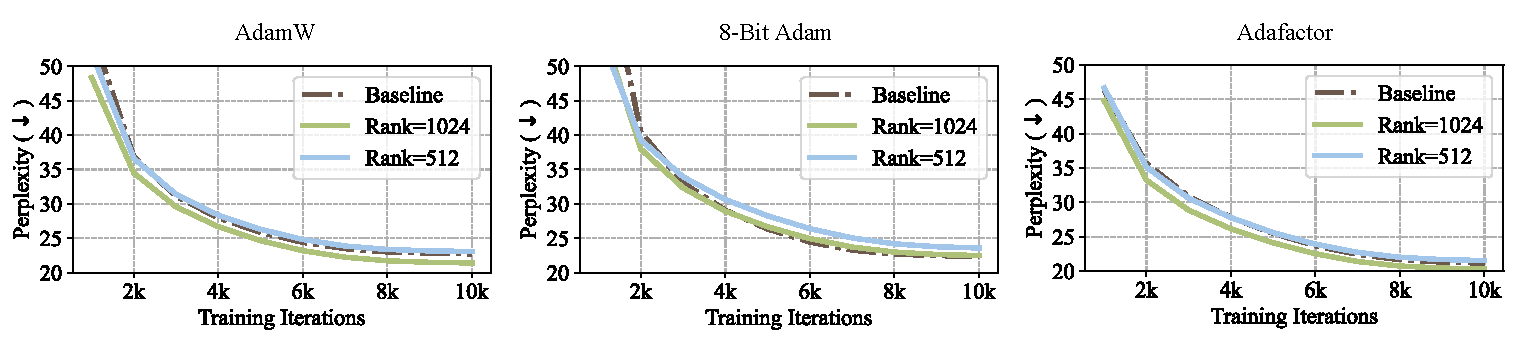
\includegraphics[width=\linewidth]{figures/train_curve.pdf}
    \vspace{-7mm}
    \caption{\small{Applying \lowrank{} to different optimizers for pre-training LLaMA 1B on C4 dataset for 10K steps. Validation perplexity over training steps is reported. We apply \lowrank{} to each optimizer with the rank of 512 and 1024, where the 1B model dimension is 2048. }}
    \vspace{-3mm}
    \label{fig:compare_optimizer}
\end{figure*}

\paragraph{Pre-training on C4.}
To evaluate its performance, we apply \lowrank{} to train LLaMA-based large language models on the C4 dataset. 
C4 dataset is a colossal, cleaned version of Common Crawl's web crawl corpus, which is mainly intended to pre-train language models and word representations \citep{raffelExploringLimitsTransfer2023}.
To best simulate the practical pre-training scenario, we train without data repetition over a sufficiently large amount of data, across a range of model sizes up to 7 Billion parameters.
\paragraph{Architecture and hyperparameters.}
We follow the experiment setup from \citet{lialinReLoRAHighRankTraining2023}, which adopts a LLaMA-based\footnote[3]{LLaMA materials in our paper are subject to LLaMA community license.} architecture with RMSNorm and SwiGLU activations \citep{zhangRootMeanSquare2019,shazeerGLUVariantsImprove2020,touvronLlamaOpenFoundation2023}. 
For each model size, we use the same set of hyperparameters across methods, except the learning rate.
We run all experiments with BF16 format to reduce memory usage, and we tune the learning rate for each method under the same amount of computational budget and report the best performance.
The details of our task setups and hyperparameters are provided in the appendix.
\paragraph{Fine-tuning on GLUE tasks.}
GLUE is a benchmark for evaluating the performance of NLP models on a variety of tasks, including sentiment analysis, question answering, and textual entailment \citep{wangGLUEMultiTaskBenchmark2019}.
We use GLUE tasks to benchmark \lowrank{} against LoRA for memory-efficient fine-tuning.

\subsection{Comparison with Existing Low-Rank Methods}

We first compare \lowrank{} with existing low-rank methods using Adam optimizer across a range of model sizes.
\paragraph{Full-Rank}
Our baseline method that applies Adam optimizer with full-rank weights and optimizer states.
\paragraph{Low-Rank}
We also evaluate a traditional low-rank approach that represents the weights by learnable low-rank factorization: $W = BA$ \citep{kamalakaraExploringLowRank2022}.
\paragraph{LoRA}
\citet{huLoRALowRankAdaptation2021} proposed LoRA to fine-tune pre-trained models with low-rank adaptors: $W = W_0 + BA$, where $W_0$ is fixed initial weights and $BA$ is a learnable low-rank adaptor. In the case of pre-training, $W_0$ is the full-rank initialization matrix.
We set LoRA alpha to 32 and LoRA dropout to 0.05 as their default settings.
\paragraph{ReLoRA}
\citet{lialinReLoRAHighRankTraining2023} proposed ReLoRA, a variant of LoRA designed for pre-training, which periodically merges $BA$ into $W$, and initializes new $BA$ with a reset on optimizer states and learning rate. ReLoRA requires careful tuning of merging frequency, learning rate reset, and optimizer states reset. We evaluate ReLoRA without a full-rank training warmup for a fair comparison.


For \lowrank{}, we set subspace frequency $T$ to 200 and scale factor $\alpha$ to 0.25 across all model sizes in Table \ref{tab:lora_compare_llama}.
For each model size, we pick the same rank $r$ for all low-rank methods, and we apply them to all multi-head attention layers and feed-forward layers in the models.
We train all models using Adam optimizer with the default hyperparameters (e.g., $\beta_1=0.9$, $\beta_2=0.999$, $\epsilon=10^{-8}$).
We also estimate the memory usage based on BF16 format, including the memory for weight parameters and optimizer states.
As shown in Table~\ref{tab:lora_compare_llama}, \lowrank{} outperforms other low-rank methods and achieves comparable performance to full-rank training.
We note that for 1B model size, \lowrank{} even outperforms full-rank baseline when $r=1024$ instead of $r=512$.
Compared to LoRA and ReLoRA, \lowrank{} requires less memory for storing model parameters and optimizer states. 
A detailed training setting of each model and memory estimation for each method are in the appendix.

\subsection{\lowrank{} with Memory-Efficient Optimizers}
We demonstrate that \lowrank{} can be applied to various learning algorithms, especially memory-efficient optimizers, to further reduce the memory footprint.
We apply \lowrank{} to AdamW, 8-bit Adam, and Adafactor optimizers \citep{shazeerAdafactorAdaptiveLearning, loshchilovDecoupledWeightDecay2019,dettmers8bitOptimizersBlockwise2021}.
We consider Adafactor with first-order statistics to avoid performance degradation.

We evaluate them on LLaMA 1B architecture with 10K training steps, and we tune the learning rate for each setting and report the best performance.
As shown in Fig.~\ref{fig:compare_optimizer}, applying \lowrank{} does not significantly affect their convergence.
By using \lowrank{} with a rank of 512, the memory footprint is reduced by up to 62.5\%, on top of the memory savings from using 8-bit Adam or Adafactor optimizer.
Since 8-bit Adam requires less memory than others, we denote 8-bit \lowrank{} as \lowrank{} with 8-bit Adam, and use it as the default method for the following experiments on 7B model pre-training and memory measurement.


\subsection{Scaling up to LLaMA 7B Architecture}
Scaling ability to 7B models is a key factor for demonstrating if \lowrank is effective for practical LLM pre-training scenarios.
We evaluate \lowrank{} on an LLaMA 7B architecture with an embedding size of 4096 and total layers of 32.
We train the model for 150K steps with 19.7B tokens, using 8-node training in parallel with a total of 64 A100 GPUs.
Due to computational constraints, we compare 8-bit \lowrank{} ($r=1024$) with 8-bit Adam with a single trial without tuning the hyperparameters.   
As shown in Table \ref{tab:7b_eval}, after 150K steps, 8-bit \lowrank{} achieves a perplexity of 14.65, comparable to 8-bit Adam with a perplexity of 14.61.



\begin{figure}[t!]
    \centering
    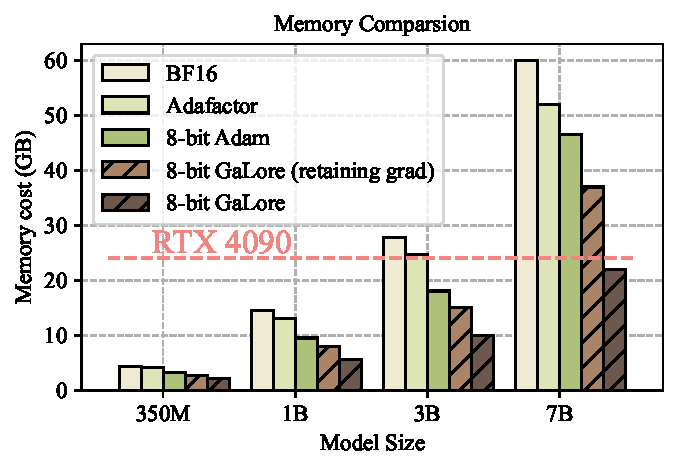
\includegraphics[width=0.9\linewidth]{figures/memory.pdf}
    \vspace{-4.5mm}
    \caption{\small{Memory usage for different methods at various model sizes, evaluated with a token batch size of 256. 8-bit \lowrank{} (retaining grad) disables per-layer weight updates but stores weight gradients during training.
    }}
    \vspace{-4mm}
    \label{fig:memory_vs_model_size}
\end{figure}


\subsection{Memory-Efficient Fine-Tuning}
\lowrank{} not only achieves memory-efficient pre-training but also can be used for memory-efficient fine-tuning.
We fine-tune pre-trained RoBERTa models on GLUE tasks using \lowrank{} and compare its performance with a full fine-tuning baseline and LoRA.
We use hyperparameters from \citet{huLoRALowRankAdaptation2021} for LoRA and tune the learning rate and scale factor for \lowrank{}.
As shown in Table~\ref{tab:fine_tuning}, \lowrank{} achieves better performance than LoRA on most tasks with less memory footprint.
This demonstrates that \lowrank{} can serve as a full-stack memory-efficient training strategy for both LLM pre-training and fine-tuning.

\begin{table}[t]
    \caption{\small Evaluating \lowrank{} for memory-efficient fine-tuning on GLUE benchmark using pre-trained RoBERTa-Base. We report the average score of all tasks.}
    \label{tab:fine_tuning}
    \centering
    \resizebox{\linewidth}{!}{%
    \begin{tabular}{l|c|cccccccc|c}
    \toprule
               & \textbf{Memory} & \textbf{CoLA} & \textbf{STS-B} & \textbf{MRPC} & \textbf{RTE} & \textbf{SST2} & \textbf{MNLI} & \textbf{QNLI} & \textbf{QQP} & \textbf{Avg} \\
    \midrule
    Full Fine-Tuning & 747M & 62.24 & 90.92 & 91.30 & 79.42 & 94.57 & 87.18 & 92.33 & 92.28 & 86.28 \\
    \midrule
    \textbf{\lowrank{} (rank=4)} & 253M & 60.35 & \textbf{90.73} & \textbf{92.25} & \textbf{79.42} & \textbf{94.04} & \textbf{87.00} & \textbf{92.24} & 91.06 & \textbf{85.89} \\
    LoRA (rank=4) & 257M & \textbf{61.38} & 90.57 & 91.07 & 78.70  & 92.89 & 86.82 & 92.18 & \textbf{91.29} & 85.61 \\
    \midrule
    \textbf{\lowrank{} (rank=8)} & 257M & 60.06 & \textbf{90.82} & \textbf{92.01} & \textbf{79.78} & \textbf{94.38} & \textbf{87.17} & 92.20 & 91.11 & \textbf{85.94} \\
    LoRA (rank=8) & 264M & \textbf{61.83} & 90.80 & 91.90 & 79.06  & 93.46 & 86.94 & \textbf{92.25} & \textbf{91.22} & 85.93 \\
    \bottomrule
    \end{tabular}
    }
    \vskip -0.1in
\end{table}





\subsection{Measurement of Memory and Throughput}
\label{sec:memory_measure}
While Table~\ref{tab:lora_compare_llama} gives the theoretical benefit of \lowrank{} compared to other methods in terms of memory usage, we also measure the actual memory footprint of training LLaMA models by various methods, with a token batch size of 256. 
The training is conducted on a single device setup without activation checkpointing, memory offloading, and optimizer states partitioning \citep{rajbhandariZeROMemoryOptimizations2020}.

\textbf{Training 7B models on consumer GPUs with 24G memory.} As shown in Fig.~\ref{fig:memory_vs_model_size}, 8-bit \lowrank{} requires significantly less memory than BF16 baseline and 8-bit Adam, and only requires 22.0G memory to pre-train LLaMA 7B with a small per-GPU token batch size (up to 500 tokens). This memory footprint is within 24GB VRAM capacity of a single GPU such as NVIDIA RTX 4090.
In addition, when activation checkpointing is enabled, per-GPU token batch size can be increased up to 4096. While the batch size is small per GPU, it can be scaled up with data parallelism, which requires much lower bandwidth for inter-GPU communication, compared to model parallelism. Therefore, it is possible that \lowrank{} can be used for elastic training~\cite{linDynamicMinibatchSGD2019} 7B models on consumer GPUs such as RTX 4090s. %

Specifically, we present the memory breakdown in Fig.~\ref{fig:memory_breakdown}.
It shows that 8-bit \lowrank{} reduces 37.92G (63.3\%) and 24.5G (52.3\%) total memory compared to BF16 Adam baseline and 8-bit Adam, respectively.
Compared to 8-bit Adam, 8-bit \lowrank{} mainly reduces the memory in two parts: (1) low-rank gradient projection reduces 9.6G (65.5\%) memory of storing optimizer states, and (2) using per-layer weight updates reduces 13.5G memory of storing weight gradients.

\textbf{Throughput overhead of \lowrank{}.} We also measure the throughput of the pre-training LLaMA 1B model with 8-bit \lowrank{} and other methods, where the results can be found in the appendix.
Particularly, the current implementation of 8-bit \lowrank{} achieves 1019.63 tokens/second, which induces 17\% overhead compared to 8-bit Adam implementation. 
Disabling per-layer weight updates for \lowrank{} achieves 1109.38 tokens/second, improving the throughput by 8.8\%. We note that our results do not require offloading strategies or checkpointing, which can significantly impact training throughput. 
We leave optimizing the efficiency of \lowrank{} implementation for future work.





\vspace{-2mm}
\section{Ablation Study}
\paragraph{How many subspaces are needed during pre-training?}

We observe that both too frequent and too slow changes of subspaces hurt the convergence, as shown in Fig.~\ref{fig:ablation} (left). The reason has been discussed in Sec.~\ref{sec:composition-subspace}. In general, for small $r$, the subspace switching should happen more to avoid wasting optimization steps in the wrong subspace, while for large $r$ the gradient updates cover more subspaces, providing more cushion. 


\begin{figure}
    \centering
        
    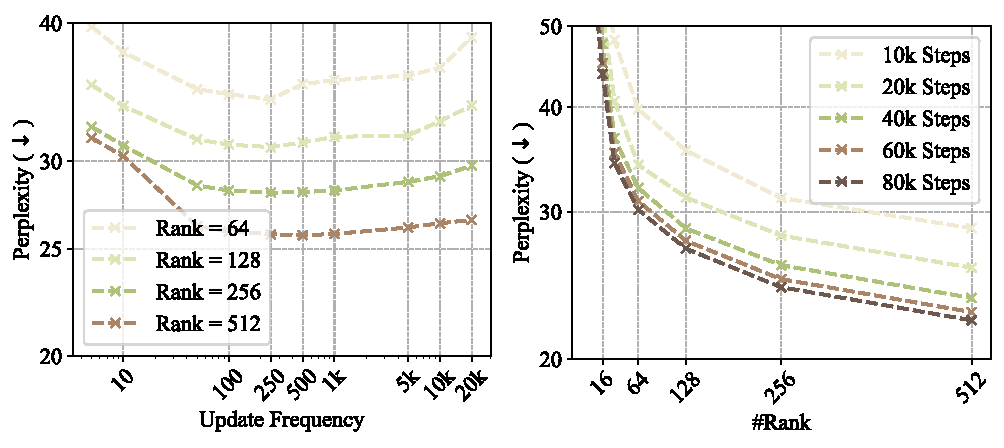
\includegraphics[width=\linewidth]{figures/files/ablation.pdf}
    \caption{\small{Ablation study of \lowrank{} on 130M models. \textbf{Left:} varying subspace update frequency $T$. \textbf{Right:} varying subspace rank and training iterations.}}
    \vspace{-7mm}
    \label{fig:ablation}
\end{figure} 


\paragraph{How does the rank of subspace affect the convergence?}
Within a certain range of rank values, decreasing the rank only slightly affects the convergence rate, causing a slowdown with a nearly linear trend.
As shown in Fig.~\ref{fig:ablation} (right), training with a rank of 128 using 80K steps achieves a lower loss than training with a rank of 512 using 20K steps.
This shows that \lowrank{} can be used to trade-off between memory and computational cost.
In a memory-constrained scenario, reducing the rank allows us to stay within the memory budget while training for more steps to preserve the performance.


